
\documentclass{article}
\usepackage[utf8]{inputenc}
\usepackage[spanish.mexico]{babel}
%\title{Dispositivos}
\author{Pablo Vivar Colina}
%\date{Septiembre 2017}

\usepackage{natbib}
\usepackage{graphicx}

%Circuitos
\usepackage{tikz}

\usepackage[american voltages, american currents,siunitx]{circuitikz}

%Diagrama de bloques

\usetikzlibrary{shapes.geometric, arrows}

\tikzstyle{startstop} = [rectangle, rounded corners, minimum width=3cm, minimum height=1cm,text centered, draw=black, fill=red!30]
\tikzstyle{io} = [trapezium, trapezium left angle=70, trapezium right angle=110, minimum width=3cm, minimum height=1cm, text centered, draw=black, fill=blue!30]
\tikzstyle{process} = [rectangle, minimum width=3cm, minimum height=1cm, text centered, draw=black, fill=orange!30]
\tikzstyle{decision} = [diamond, minimum width=3cm, minimum height=1cm, text centered, draw=black, fill=green!30]


\tikzstyle{arrow} = [thick,->,>=stealth]
%###MIO###
\tikzstyle{point} = [circle,(0.5cm),minimum with=1cm,draw=black,fill=black!50]



%Plotting

\usepackage{pgfplots}
\pgfplotsset{width=10cm,compat=1.9} 
 \usepgfplotslibrary{external}
\tikzexternalize 

%#####Fracciones DIAGONALES :B #####

\usepackage{amsmath}
\usepackage{mathtools}

%running fraction with slash - requires math mode.
\newcommand*\rfrac[2]{{}^{#1}\!/_{#2}}


%\maketitle

%\usepackage[top=2cm,bottom=2cm,left=1cm,right=1cm]{geometry}


\begin{titlepage}
     \begin{center}
	
\includegraphics[width=0.09\textwidth]{UNAM}\Large Universidad Nacional Autónoma de México
        	
\includegraphics[width=0.09\textwidth]{FI}\\[1cm]
        \Large Facultad de Ingeniería\\[1cm]
       % \Large División de Ciencias Básicas\\[1cm]
         \Large Laboratorio de Fundamentos de Control(6655)\\[1cm]
         %la clave antes era:4314
         \footnotesize Profesor: Salcedo Ubilla María Leonor Ing.\\[1cm]
        \footnotesize Semestre 2019-1\\[1cm]
        
       

        \Large Práctica No. 1\\[1cm]
        
           

\Large Introdcción MATLAB
        
         %Texto a la derecha
          \begin{flushright}
\footnotesize  Grupo 2\\[0.5cm]
\footnotesize Brigada: 4\\[0.5cm]
\footnotesize Rodrigo Adrián Martínez López\\[0.5cm]
\footnotesize Vivar Colina Pablo\\[0.5cm]
 \end{flushright}
    %Texto a la izquierda
          \begin{flushleft}
        \footnotesize Ciudad Universitaria Agosto de 2018.\\
          \end{flushleft}
         
          
        %\vfill
        %\today
   \end{center}
\end{titlepage}
 %agregar portada

\begin{document}



\tableofcontents  % Write out the Table of Contents

\listoffigures  % Write out the List of Figures


\section{Marco Teórico}

\section{Ruido}

La mayoría de las aplicaciones se tiene o considera al ruido r como aditivo, esto es para la señal enviada $s$ se tiene que:\citep{Capitulo1SC}\\

\begin{equation}
    x_r=s+r
\end{equation}

Donde $x_r$ es la señal recibida.\citep{Capitulo1SC}\\

El ruido natural tiende a ser gaussiano, esto es, su densidad es:\citep{Capitulo1SC}

\begin{equation}
    p(n)=\frac{1}{\sqrt{2 \pi \sigma_n}} e^{-\frac{(m-n_m)^2}{2 \sigma_n^2}}
\end{equation}

\begin{figure}[h!]
    \centering
    
   
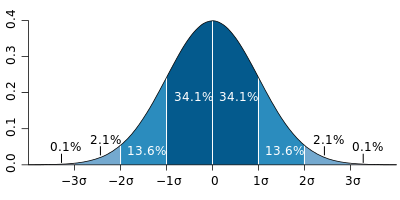
\includegraphics[width=0.6\textwidth]{Imagenes/Standard_deviation_diagram.png}
\caption{ La distribución Normal suele conocerse como la "campana de Gauss".}
    \label{fig:distNorm}
 
\end{figure}


Refiriéndonos a la distribución normal, la cual podemos apreciar en la figura \ref{fig:distNorm} tenemos que:\citep{DistribucionNormal}\\

\begin{itemize}
    \item $\sigma^2$ es la varianza
    \item $n_m$ es la moda
\end{itemize}


El ruido más común es blanco y se define como aquel de densidad de potencia constante.\citep{Capitulo1SC}\\

\begin{equation}
    G_n(f)=\frac{N_0}{2}
\end{equation}

entonces:\\


\begin{equation}
    R_n(\tau)=\frac{N_0}{2} \delta (\tau)
\end{equation}

El ruido térmico es blanco, aditivo y gaussiano, como este ruido esta presente en todos los sistemas de comunicaciones, se utilizan sus características para modelar ruido en comunicaciones.\citep{Capitulo1SC}




\section{Desarrollo}

\subsection{Diagrama de bloques}



\begin{figure}[h!]
    \centering
    \begin{tikzpicture}[node distance=4cm]

%startstop-->ROJO
\node (start) [process] {Generador de señales};



\node (ReP) [process, right of=start] {Red en Prueba};



\node (Volt) [process, right of=ReP, ] {Voltímetro};
%yshift=-0.5cm

\node (Canal1) [process,yshift=-2cm,above of=Canal2] {Canal 1 Osciloscopio};

\node (Canal2) [process, above,yshift=-2cm, above of=Volt] {Canal 2 Osciloscopio};

\node (AeE) [process,yshift=2cm, below of=Volt] {Analizador de Espectros};


%Línea inicio a red en prueba
\draw [arrow] (start) -- (ReP);


%Línea de red en prueba aVoltimetro 
\draw [arrow] (ReP) |- (Volt);

\draw [arrow] (start) --(Canal1);

\draw [arrow] (Volt) -- (Canal2);
\draw [arrow] (ReP) |- (AeE);

\end{tikzpicture}
    \caption{Sistema de pruebas}
    \label{fig:sistPruebas}
\end{figure}



\subsection{Circuito con componente no lineal y 1 señal de entrada}

Para éste experimento se utilizó una señal de entrada de 1 [kH] y se estuvieron variando las amplitudes de las señales, ésto se puede apreciar en las figura \ref{fig:SenialEspNoLin}.\\

Después se conectaron los instrumentos de medición a la salida del segundo circuito RC Y calcule nuevamente el porcentaje de distorsion.\\

Los porcentajes de distorsión para el primer filtro fueron:\\

\begin{itemize}
    \item $V_{total}$=1.377[V]
    \item $V_{fundamental}$=1.277[V]
    \item $\%Dist$=140.79
\end{itemize}

Ésto se puede apreciar en la figura \ref{}

Los porcentajes de distorsión para el segundo filtro fueron:\\

\begin{itemize}
    \item $V_{total}$=617 [mV]
    \item $V_{fundamental}$=504 [mV]
     \item $\%Dist$=70.617
\end{itemize}





\begin{figure}[h!]
    \centering
    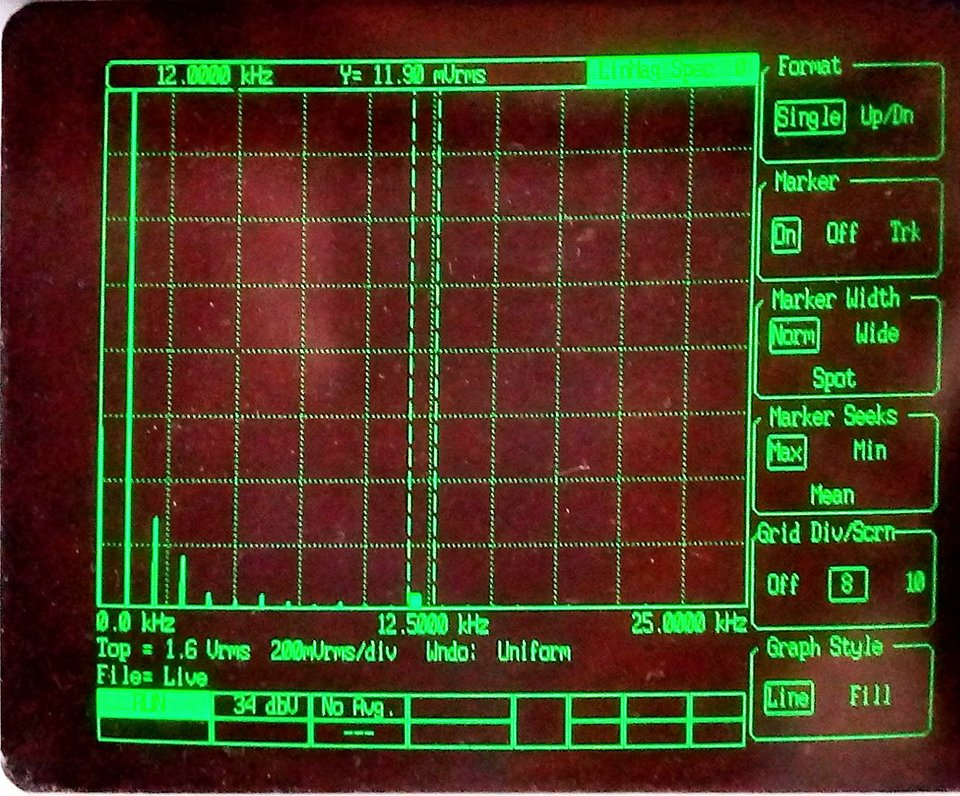
\includegraphics[width=0.5\textwidth]{Imagenes/SistComDistAlin.jpg}
    \caption{Espectro de Frecuencias dispositivo no lineal}
    \label{fig:espNoLin}
\end{figure}

Aumente la amplitud de la señal de entrada. Anote el espectro y oscilograma a la salida del amplificador. Note la distorsion armonica que se produce. Calcule el porcentaje de distorsion de la señal a la salida del amplificador. 

\begin{figure}[h!]
    \centering
    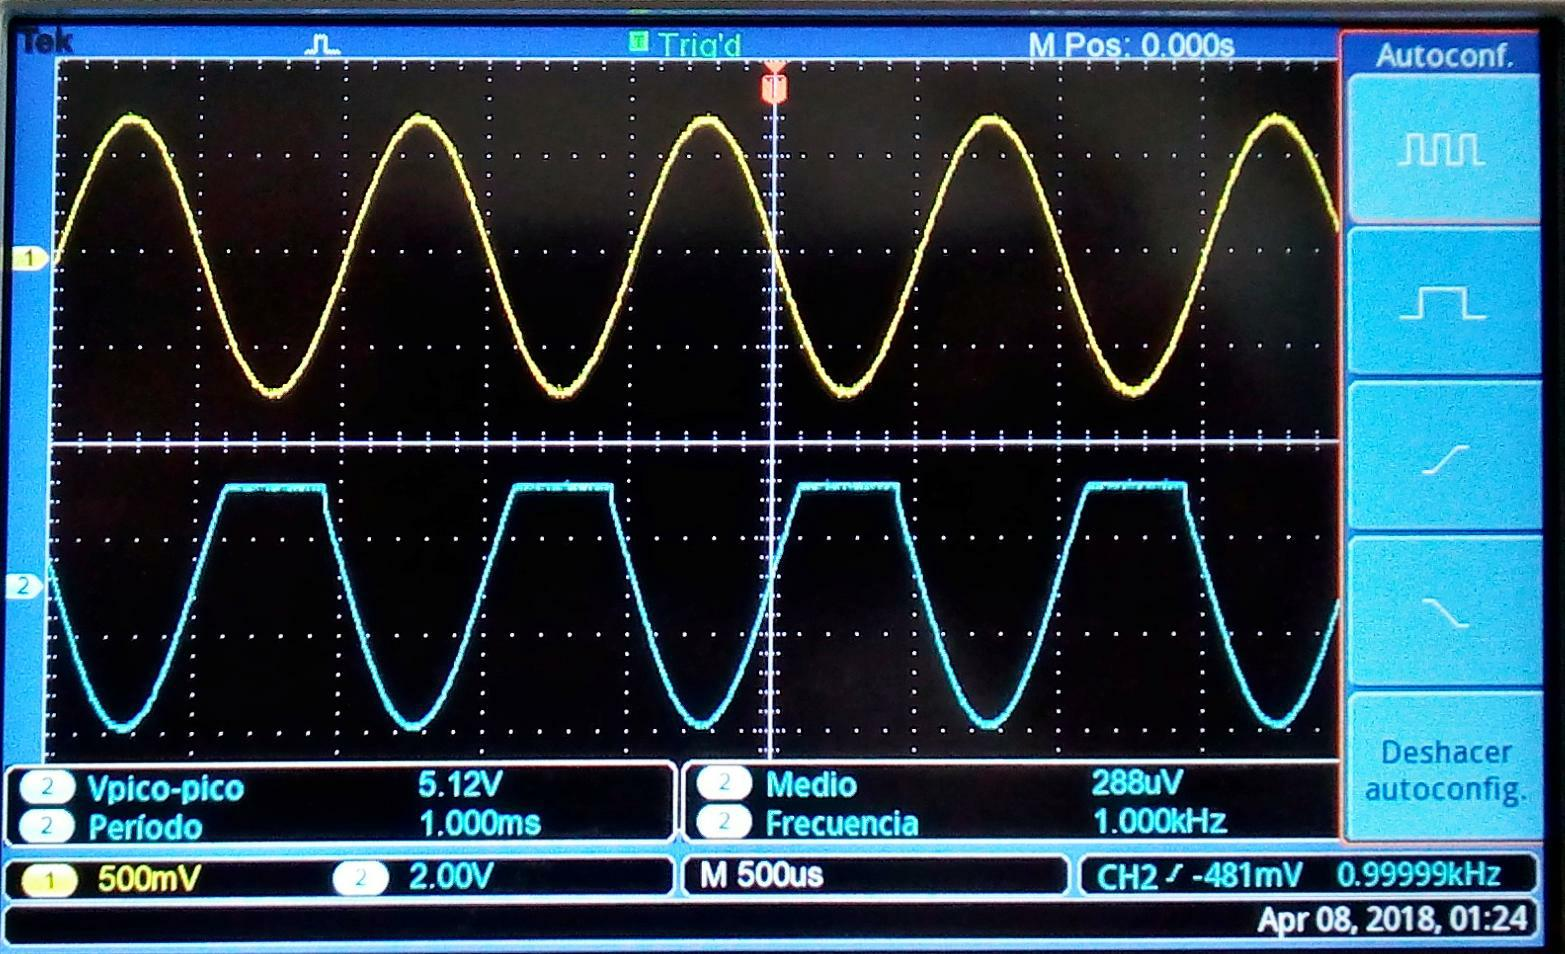
\includegraphics[width=0.5\textwidth]{Imagenes/SistComDistAlin1.jpg}
    \caption{Señales obtenidas por distosión dispositivo no lineal en frecuencias en la figura \ref{fig:espNoLin}}
    \label{fig:SenialEspNoLin}
\end{figure}

\begin{figure}[h!]
    \centering
    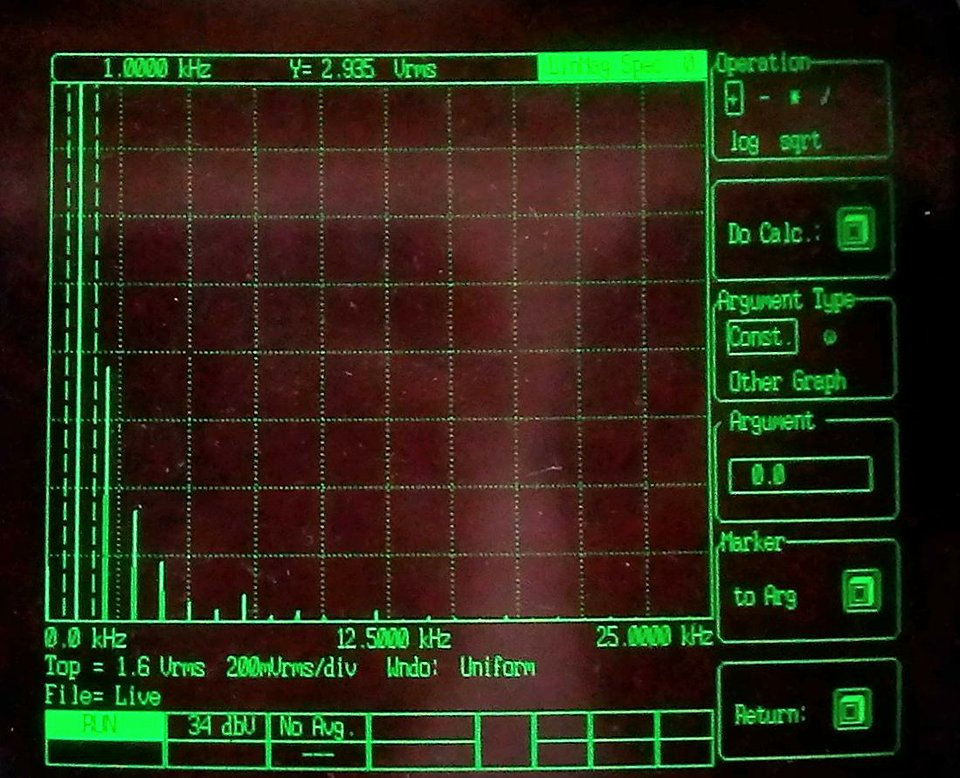
\includegraphics[width=0.5\textwidth]{Imagenes/SistComDistAlin2.jpg}
    \caption{Gráfica}
    \label{fig:grafB}
\end{figure}

\begin{figure}[h!]
    \centering
    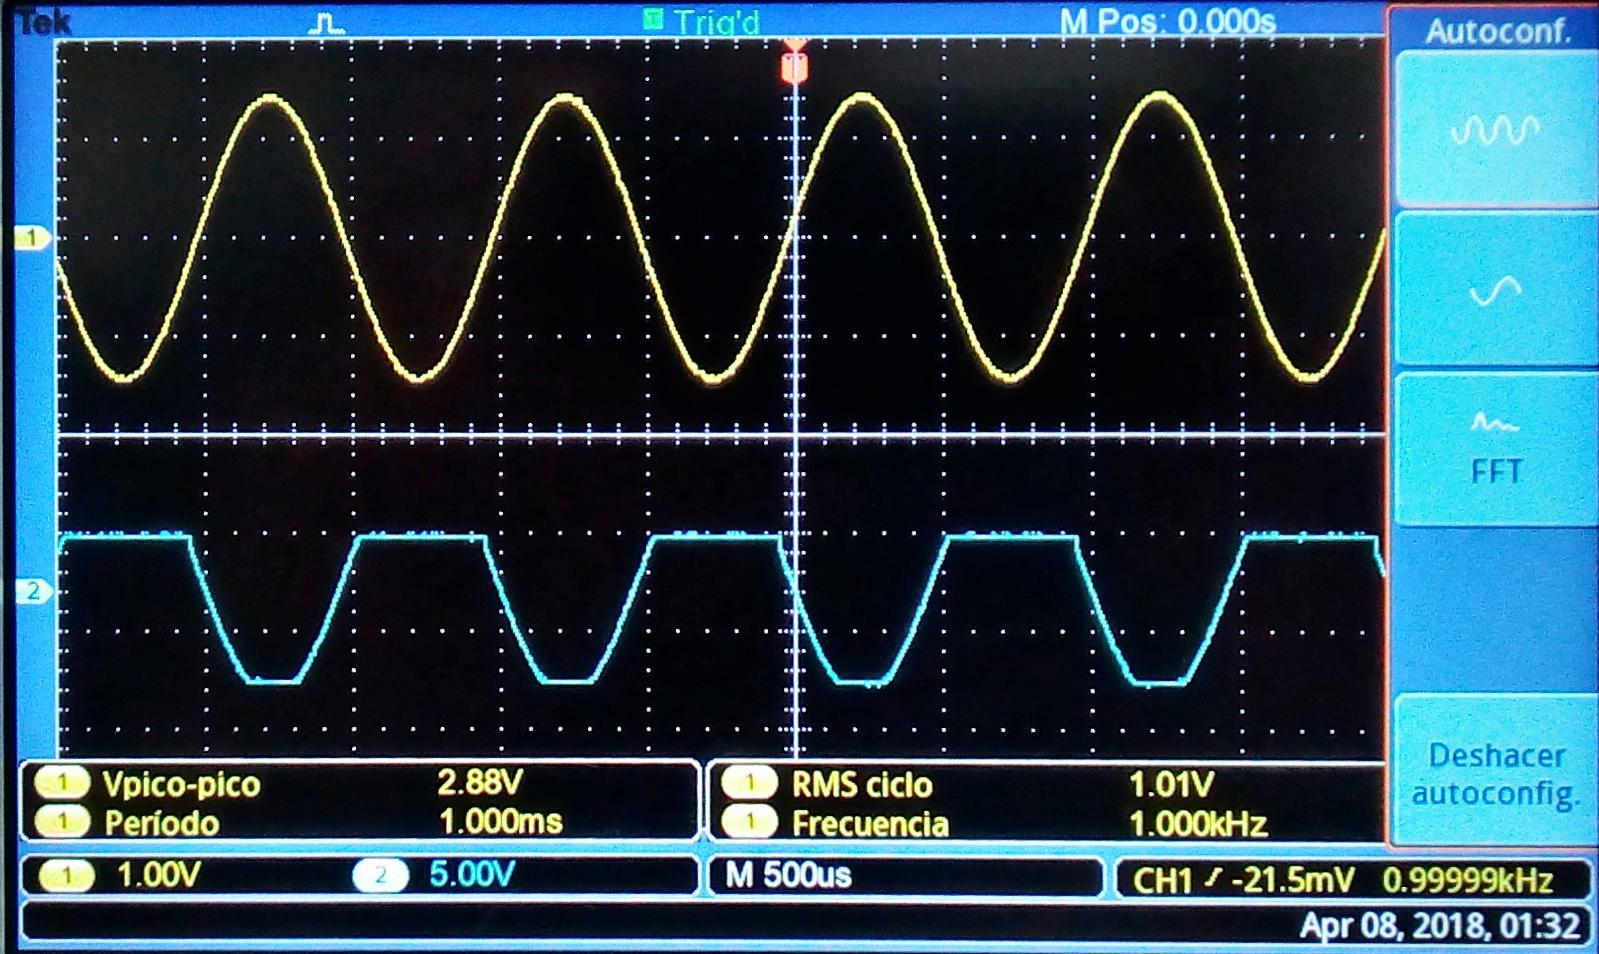
\includegraphics[width=0.5\textwidth]{Imagenes/SistComDistAlin3.jpg}
    \caption{Gráfica}
    \label{fig:grafC}
\end{figure}

\begin{figure}[h!]
    \centering
    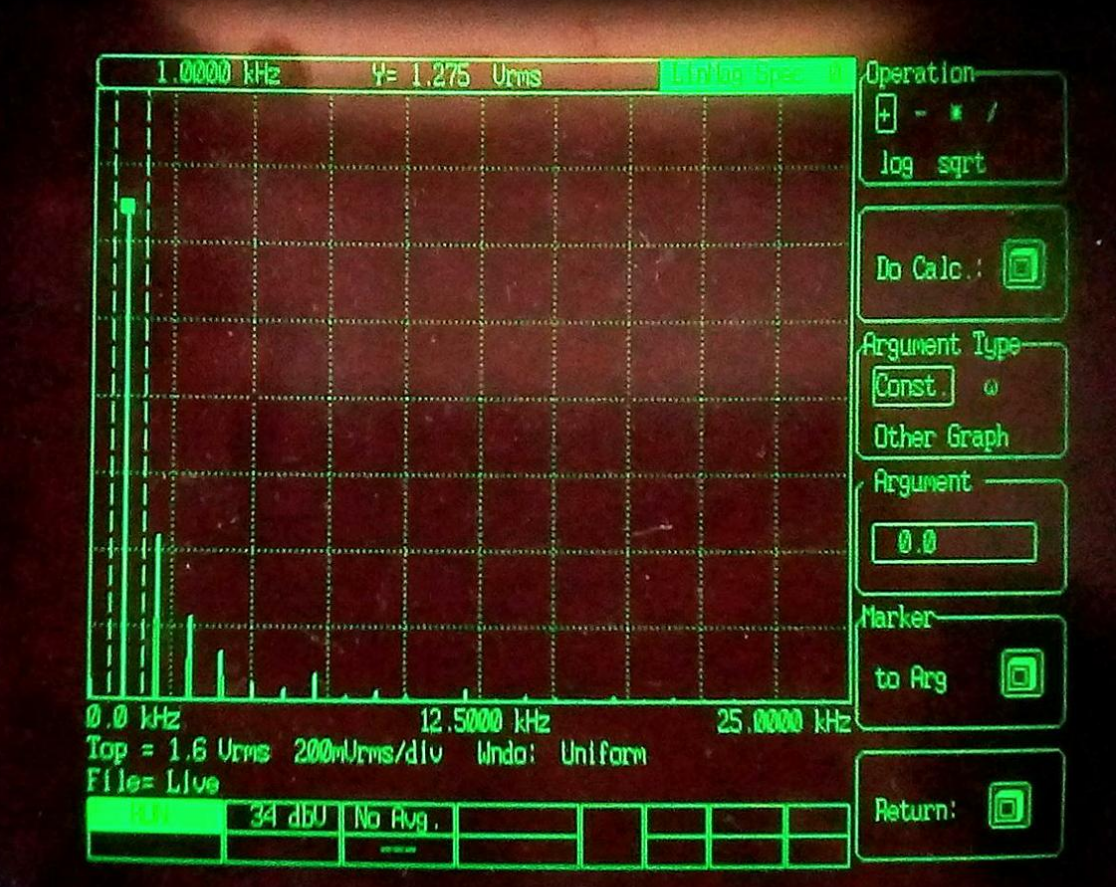
\includegraphics[width=0.5\textwidth]{Imagenes/SistComDistAlin4.png}
    \caption{Gráfica}
    \label{fig:grafA}
\end{figure}

\begin{figure}[h!]
    \centering
    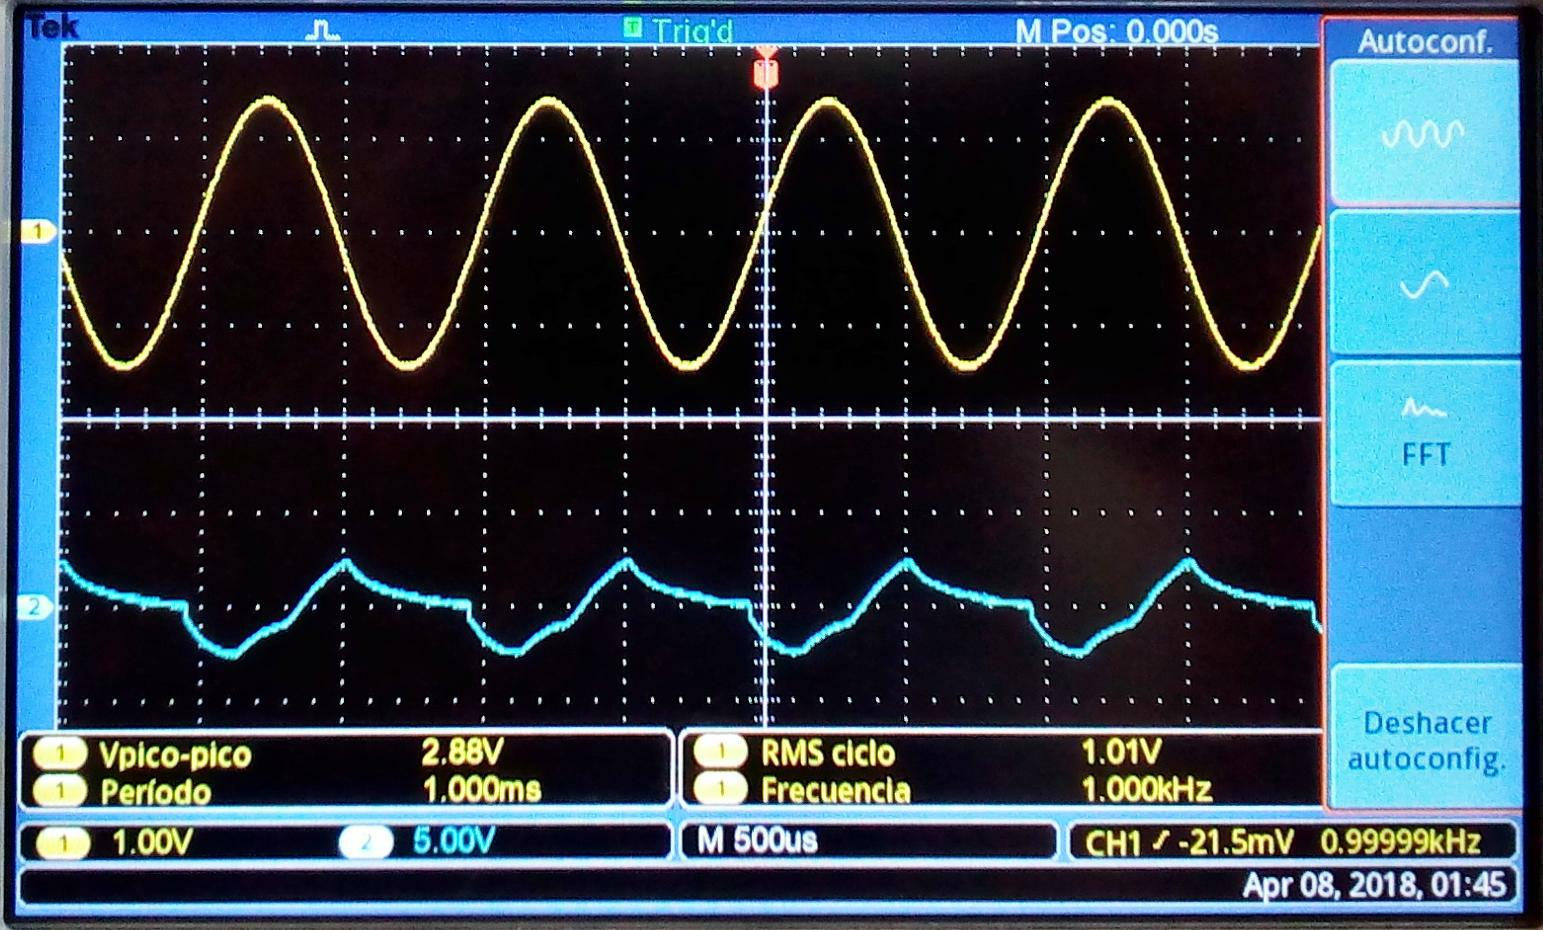
\includegraphics[width=0.5\textwidth]{Imagenes/SistComDistAlin5.jpg}
    \caption{Señales obtenidas por distosión dispositivo no lineal en frecuencias en la figura \ref{fig:espNoLin}}
    \label{fig:grafD}
\end{figure}

\begin{figure}[h!]
    \centering
    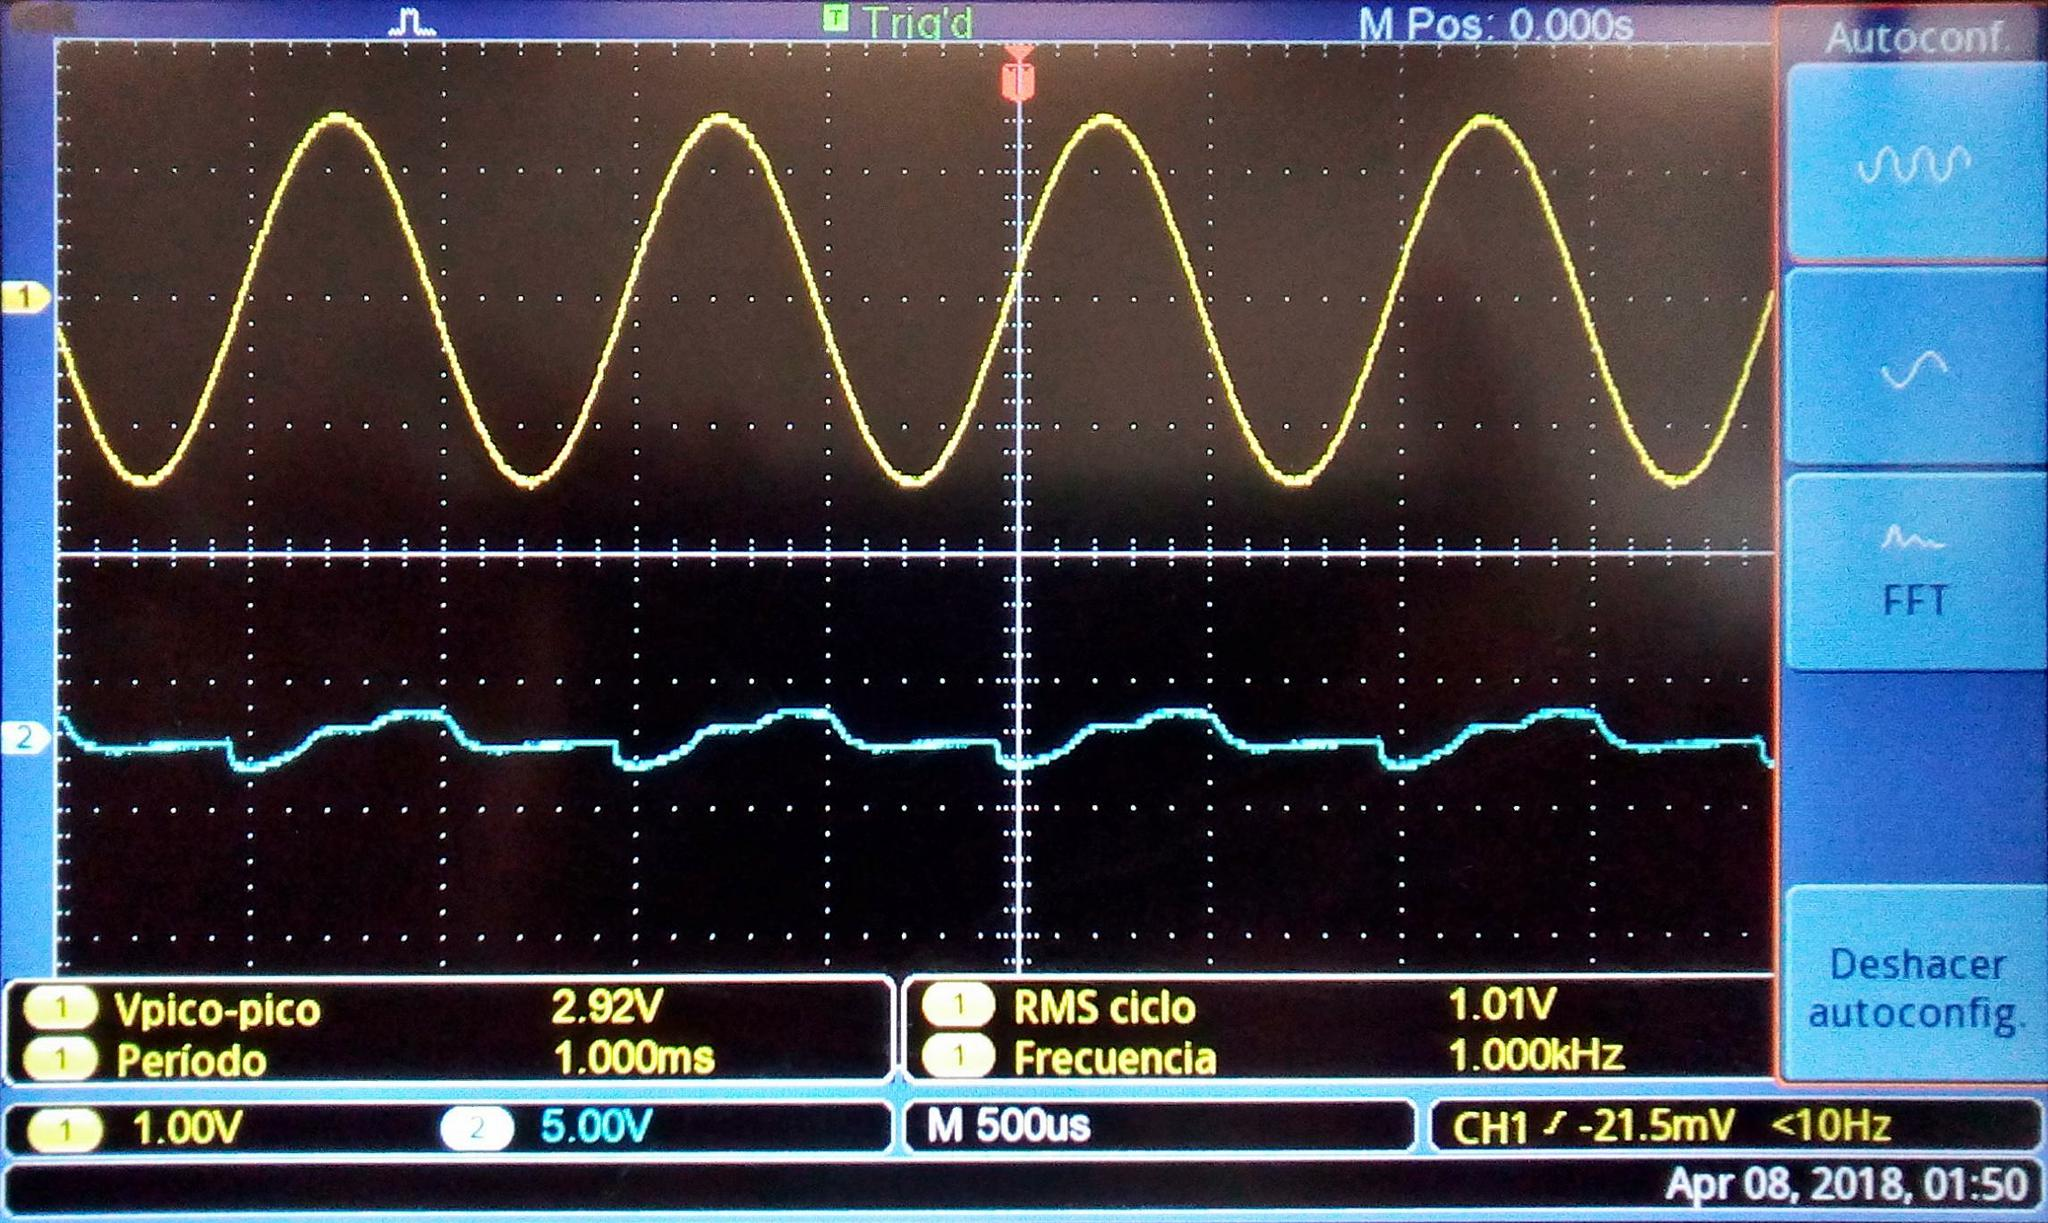
\includegraphics[width=0.5\textwidth]{Imagenes/SistComDistAlin6.jpg}
    \caption{Gráfica}
    \label{fig:grafE}
\end{figure}




\begin{figure}[h!]
    \centering
    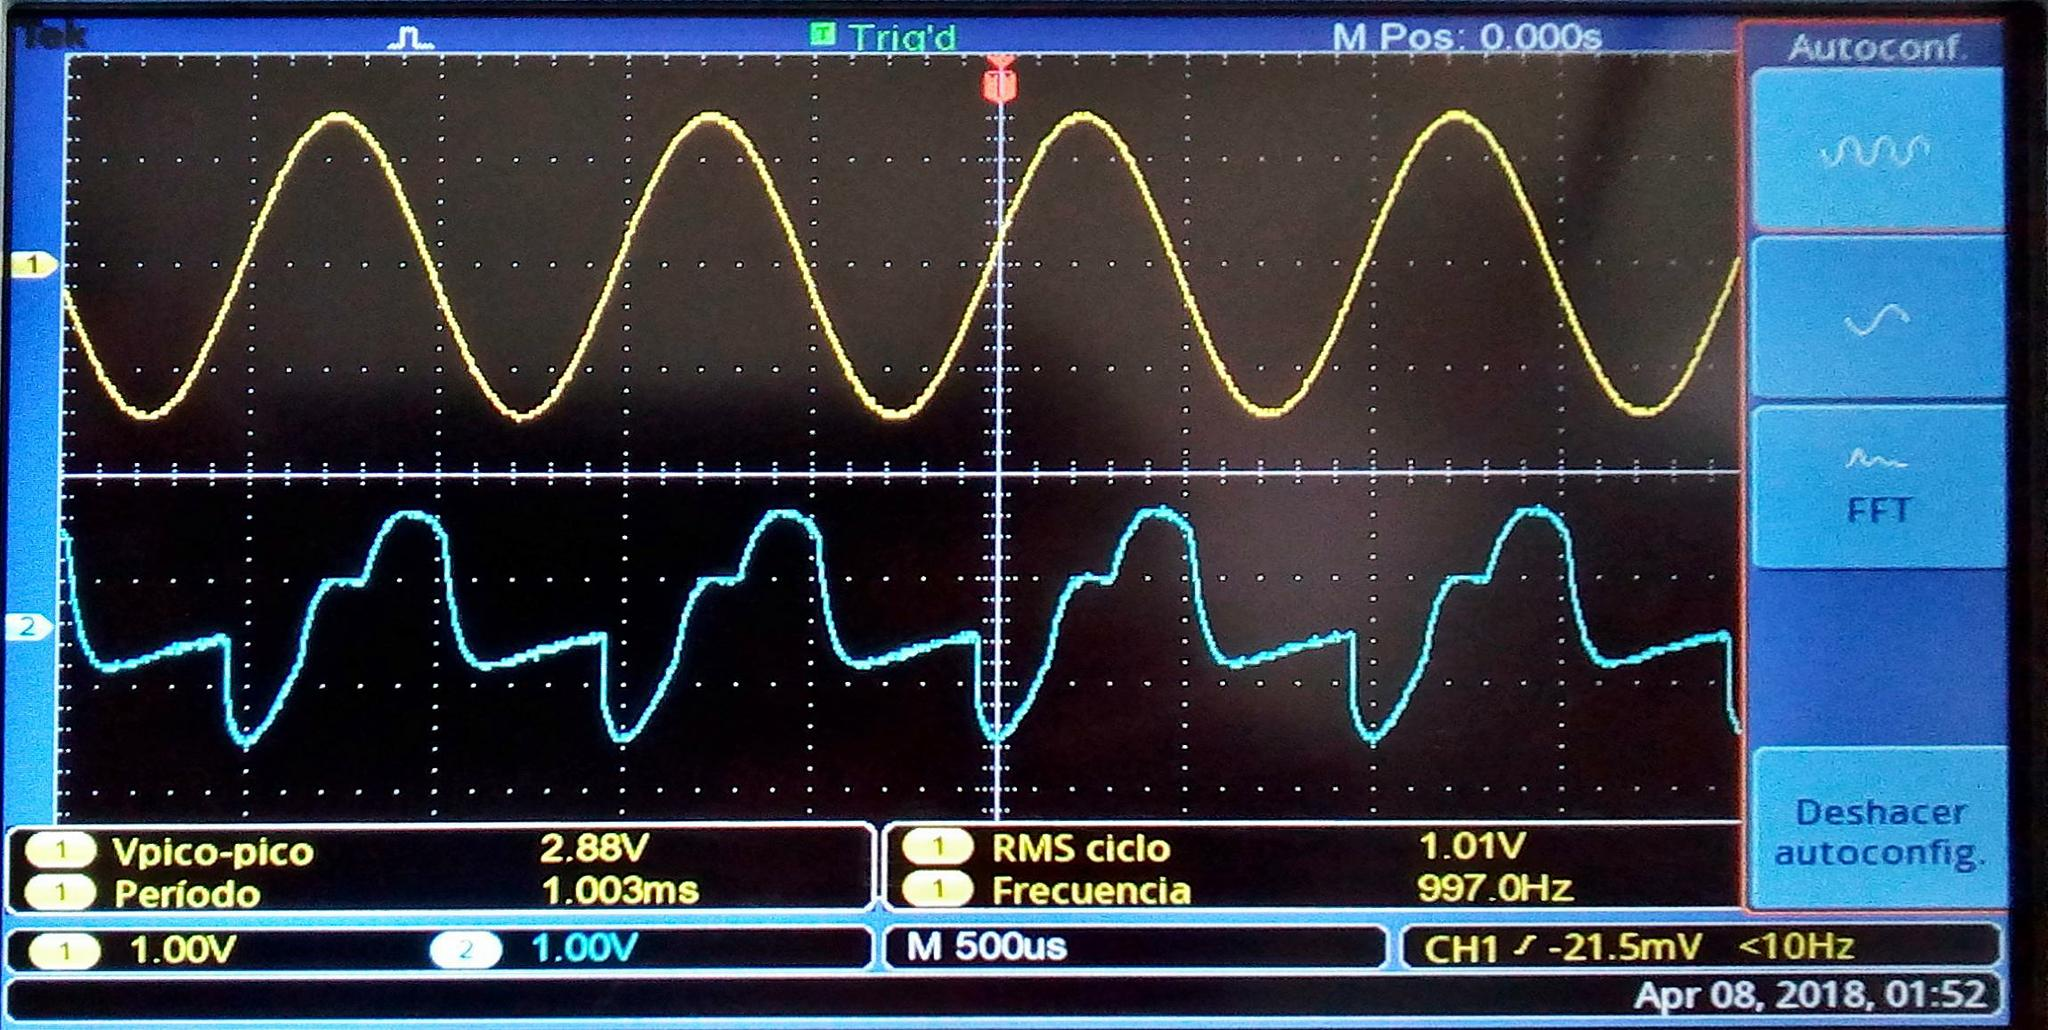
\includegraphics[width=0.5\textwidth]{Imagenes/SistComDistAlin7.jpg}
    \caption{Señales obtenidas en la salida en el filtro 1}
    \label{fig:SenialFiltro1}
\end{figure}

\subsection{Entrada de 2 señales}

Se conectaron dos señales senoidales de 1 kHz y 3.5 kHz respectivamente, a la entrada del amplificador. Anote el oscilograma y espectro de la señal a la salida del amplificador, las señales de netrada y salida se pueden apreciar en la figura \ref{fig:SenialFiltro2}

%explicando la presencia de cada línea espectral

\begin{figure}[h!]
    \centering
    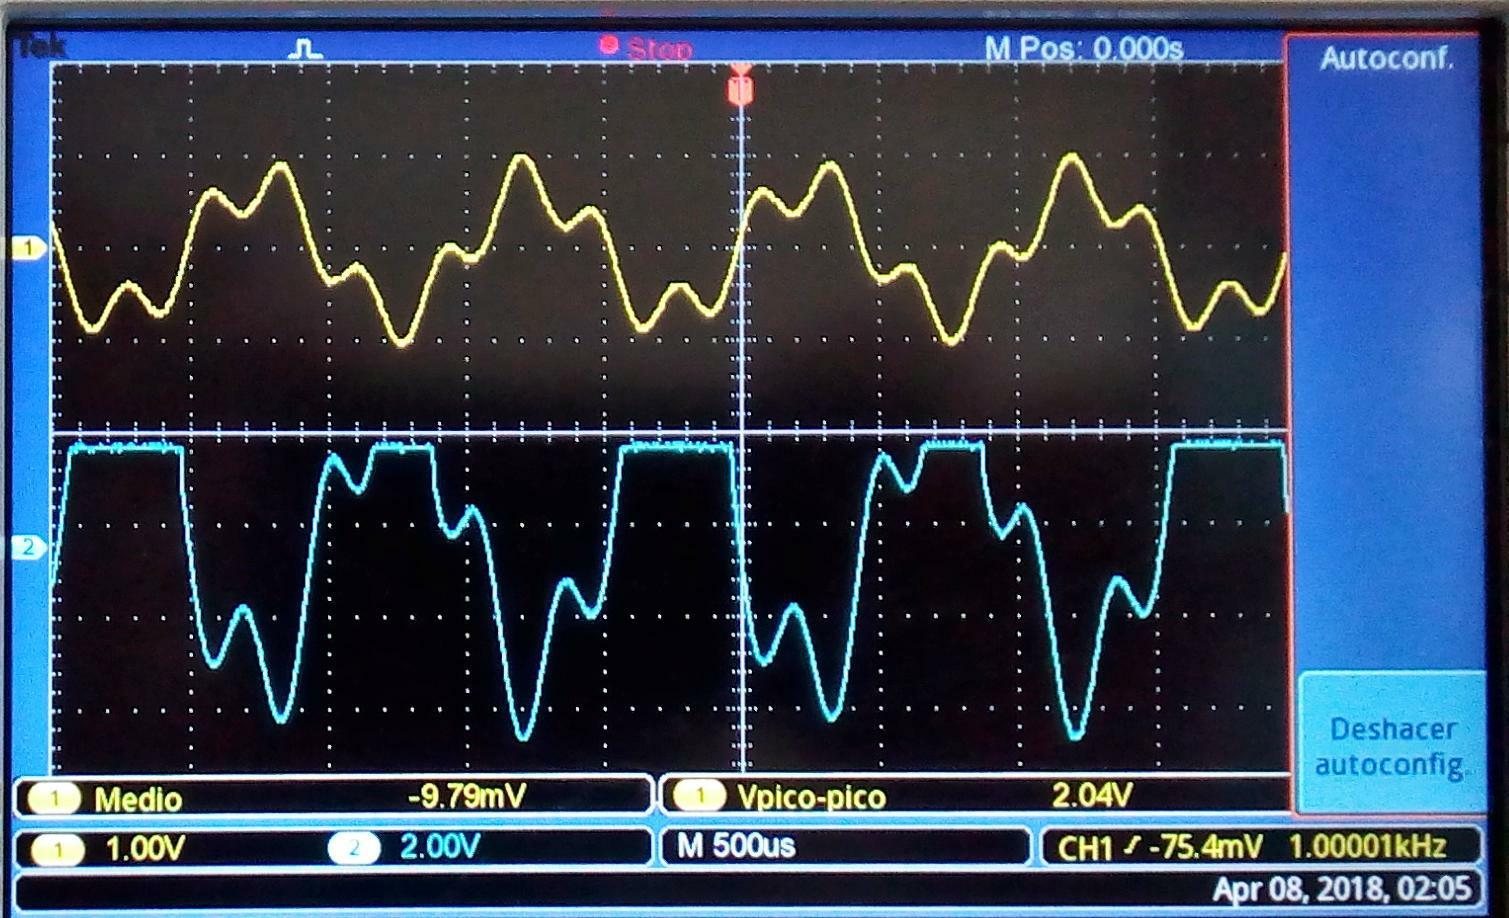
\includegraphics[width=0.5\textwidth]{Imagenes/SistComDistAlin8.jpg}
    \caption{Señales obtenidas en la salida en el filtro 2}
    \label{fig:SenialFiltro2}
\end{figure}





\begin{figure}[h!]
    \centering
    \begin{circuitikz}
    
    \draw
    
    (0,0)to[D,l=$D_1$](2,0)
    
    
    %Filtro 1
    (2,0)to[C,l=$C_1$](4,0) 
    
    (4,0)to[R,l=$R_1$](4,-2)
    
    %Filtro 2
    (4,0)to[C,l=$C_2$](6,0) 
    
    (6,0)to[R,l=$R_2$](6,-2)
    
    
    (6,0)--(8,0)
    
    (0,-2)--(8,-2)
    

   %Leyenda Filtro 2
    (5,1.3) node{Filtro 2}

    %Leyenda Filtro 1
    (3,1.3) node{Filtro 1}
    
    %Leyenda Entrada
    (0,-1) node{Entrada}
    
    %Leyenda Salida A
    (2,-0.2) node{+}
    (2,-1) node{A}
    (2,-1.8) node{-}
    
    %Leyenda Salida B
    (4.5,-0.2) node{+}
    (4.5,-0.5) node{B}
    (4.5,-1.8) node{-}
    
      %Leyenda Salida C
    (6.5,-0.2) node{+}
    (6.5,-0.5) node{C}
    (6.5,-1.8) node{-}




    ;
   
    \end{circuitikz}
    \caption{Circuito con filtros}
    \label{fig:circuitoConFiltros}
    
    \end{figure}








\section{Conclusiones Martínez Hernández Fernando}

En esta practica conocimos la distorsión que sufren las señales que se propagan en los cables telefónicos y una de las formas de corregirla, aprendimos que en la distorsión lineal solo cambia la fase y la amplitud de la entrada con respecto a la salida, mediante filtros observamos como se corregía la distorsión.

\section{Conclusiones Pablo Vivar Colina}

En la práctica se apreció la distorsión Alineal en los dispositivos y su diferente comportamiento a través de cambiar su la frecuencia de las señales de entrada, inyectar más de una señal, y cambiar los filtros a la salida señales, se verificó éste último caso en el circuito de la figura \ref{fig:circuitoConFiltros}\\


\section{Comentarios}

La distorsión de una señal es algo que se puede medir en porcentaje a partir de las señales que se están recibiendo, es importante porque para los sistemas de comuniación para conocer como cambia la señal al transmitirse y se pueda interpretar de manera correcta



\bibliographystyle{plain}
\bibliography{Referencias.bib}

\end{document}
